\section{Литературный обзор}

Экстремальные тепловые нагрузки на материал стенок установки --- одна из
основных проблем создания будущих коммерчески эффективных термоядерных
реакторов. Для строящегося ITER в 2013 году в качество основных были
выбраны~\cite{merola2015engineering} плитки состоящие из $W$ и имеющие подложку
из $CuCrZr$~\autoref{pic::Motojime_tile}, способные выдерживать нагрузки до $4.7$ МВт$/$м$^2$. Плитки,
используемые в диверторах испытывают гораздо большие тепловые нагрузки и
способны выдерживать до $20$ МВт$/$м$^2$~\cite{motojima2015iter}.
Несогласованная плитка может подвергаться нагрузкам до 15---60 раз
большим~\cite{moritz2023thermionic}. 

\begin{figure}[H]
	\centering
	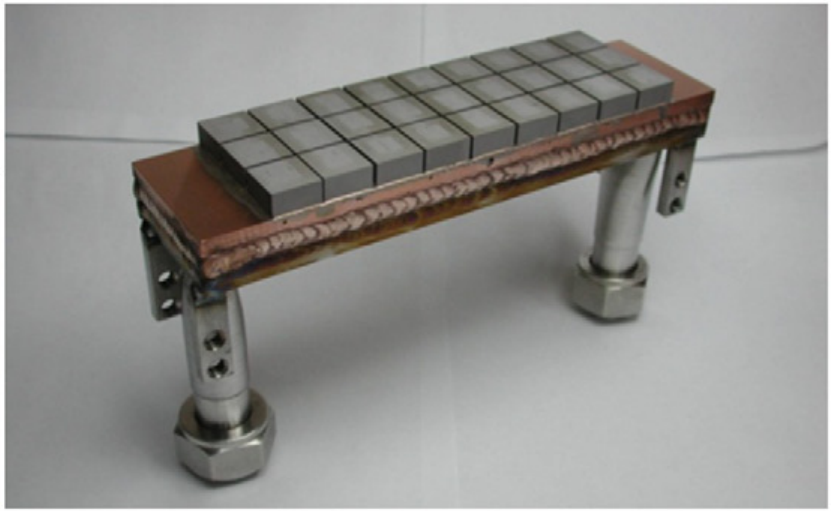
\includegraphics[width=0.7\linewidth]{material/Motojima_tile.png}
    \caption{Фотография плитки, изготовленной для использования в
    ITER~\cite{motojima2015iter}. Медная подложка содержит теплоотводные трубки с
водой.}
	\label{pic::Motojime_tile}
\end{figure}

В экспериментах на токамаке JET прохождение ПЛМ наблюдалось с частотой порядка
$f_{ELM} = 30$ Гц~\cite{coenen2015elm}. 
В ходе прохождения филаментов по поверхности плитки температура поверхности
достигает величин порядка температуры плавления$\left(T_W^{\text{melt}}\right.$ 
$\left.= 3695\text{ К }\right)$~\cite{coenen2015elm}. 
Плавление материала поверхности стенки в современных спецификациях принято как
явление не препятствующее корректной работе реактора, в то время как плавление
всего моноблока, очевидно, является недопустимым явлением\hl{поправить
цитирование: взять конкретное выступление Loarte}~\cite{soukhanovskii23rd}
Так, в работе~\cite{gunn2017surface} сделан вывод о возможности оплавления
поверхности моноблоков дивертора в ходе прохождения ПЛМ во время тестовых сценариев с
использованием $He-D$ смеси\hl{(15 МА)}. При сценариях с использованием $D-T$ смеси
плавление основной части моноблока является неизбежным явлением при прохождении
ПЛМ.

Из последствий плавления поверхностей вольфрамовых плиток можно упомянуть
возможное попадание ионов вольфрама в основной объём плазмы, что даже при малых
концентрациях (порядка $1.0\cdot10^{-5}$ от общего числа атомов\hl{где-то у
Pitts}) делает термоядерный синтез невозможным. Так же, возникают капельные
фракции --- порядка 80 мкм~\cite{coenen2015elm}.

В отсутствие ПЛМ, стационарная температура поверхности дивертора в ITER
ожидается равной $1100-2000$ К в различных областях при нагрузке $q_{tg} = 10$
МВт/м$^2$~\autoref{pic::Motojime_tile}
\begin{figure}[H]
	\centering
	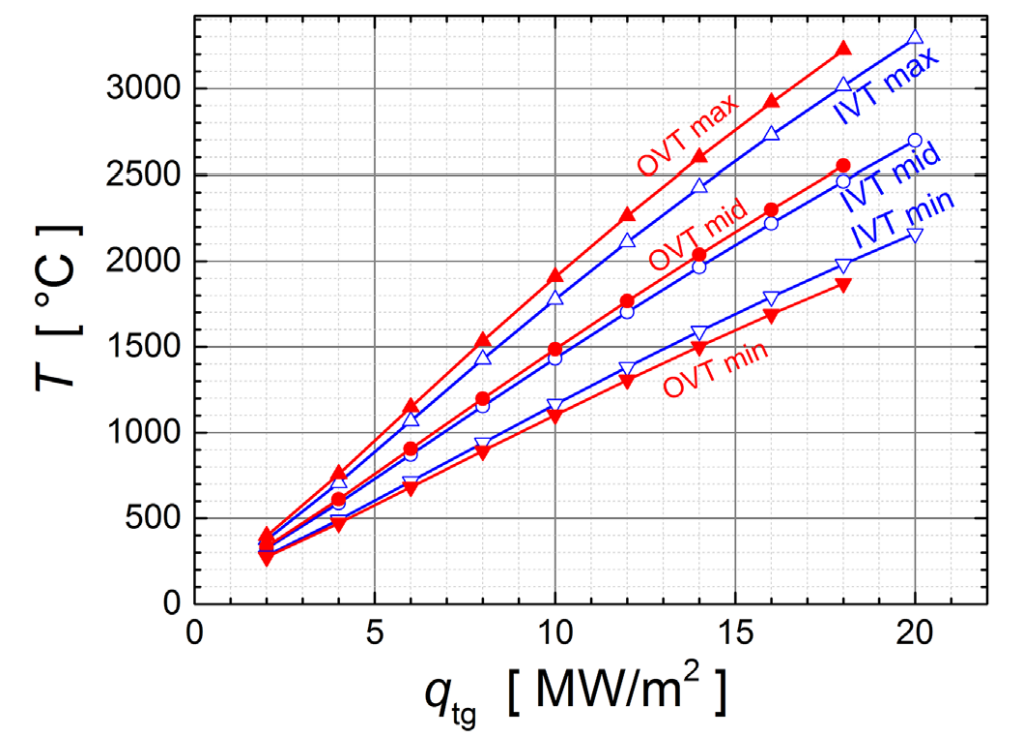
\includegraphics[width=0.7\linewidth]{material/Gunn_temperatures_qtg.png}
    \caption{Результаты моделирования температуры поверхности моноблока
    дивертора в ITER.~\cite{gunn2017surface} OVT --- внешняя вертикальная цель,
IVT --- внутренняя вертикальная цель.}
	\label{pic::Motojime_tile}
\end{figure}

Для задачи поиска значений параметров дебаевского слоя в
термоядерных установках важными являются параметры ПЛМ. ПЛМ могут иметь разные
причины возникновения и имеют соответствующую классификацию. Несмотря на это, 
их принципиальные свойства являются едиными~\cite{spolaore2017electromagnetic}.
Филаменты, являющиеся выбросом плазмы из основного объёма, имеют хорошую
проводимость\hl{порядка проводимости стали}. В соответствии с хорошо описанным
являнием вмораживания магнитных силовых линий в плазму, они являются
''проводниками'' осцилляций электромагнитного поля. На токамаке COMPASS в ходе
экспериментов наблюдались осцилляции магнитного поля~\hl{в какой точке на
стенке?} при прохождении филамента по поверхности плитки.

В работе \cite{spolaore2017electromagnetic} приводятся следующие параметры
осцилляций в ПЛМ: средняя длительность прохода ПЛМ $t_{ELM} = 0.35$ мс, осцилляции магнитного поля
имеют малую амплитуду: $\delta B \approx 0.2$ мТ $\ll~B = 1.15$ Т, но
возникающий из---за них ток через дебаевский слой
значителен~\hl{цитирование laggner с графиком для asdex upgrade?}. Частота сигнала,
распространяющегося внутри филамента имеет характерные частоты порядка
$100$---$240$ КГц~\cite{spolaore2017electromagnetic},~\cite{laggner2016high}, соответствующей характерному
значению альфвеновской частоты $\nu_A$. Отсюда, можно сделать вывод о
необходимости учёта тока смещения в дебаевском слое: найдём частоту, при которой
ток смещения становится порядка тока
проводимости~\eqref{eq::displace_current::1}.
\begin{gather}
    \cfrac{\partial \vec{B}}{\partial t} = \cfrac{4\pi}{c}\vec{j} +
    \cfrac{1}{c}\cfrac{\partial \vec{E}}{\partial t}\\
    \cfrac{1}{c}\cfrac{\partial \vec{E}}{\partial t} \sim \cfrac{\omega}{c}E
    \sim \cfrac{\omega}{c}\cfrac{j}{\sigma}
    \label{eq::displace_current::1}
\end{gather}
\begin{equation}
    \cfrac{\cfrac{\omega}{c}\cfrac{j}{\sigma}}
    {\cfrac{4\pi}{c}j}
    \sim \cfrac{\omega}{4\pi\sigma} 
    \sim \cfrac{\omega}{4\pi\cfrac{ne^2}{m_e}\cfrac{1}{\nu_e}}
    = \cfrac{\omega \nu_e}{\omega_{pe}^2} \sim 1
    \label{eq::displace_current::2}
\end{equation}
При параметрах $n_e = 10^{13}$ см$^{-3}$, $T_e = 100$ эВ, следует, что $\omega
\sim 10^{16}$ с${-1}$. Таким образом, влияние тока смещения является малозначительным,
по сравнению с током проводимости в рассматриваемых сценариях.

При температурах, достигающих температуры плавления, роль термоэлектронной
эмиссии и ее влиянии на регуляцию потоков через дебаевский слой становится
крайне значимым~\cite{takamura1998heat}. Термоэлектронная и вторичная
электронная эмиссии являются основными в экранировании потоков через слой,
ограничивая резкое уменьшение плавающего потенциала поверхности плитки при росте
температуры поверхности. Эмитированные электроны образуют виртуальный катод ---
минимум потенциала в дебаевском слое, способный ''запирать'' частицы возле
поверхности стенки и отражать недостаточно быстрые электроны, идущие со стороны
плазмы. Данное явление известно давно и было аналитически описано в классической
работе~\cite{langmuir1913effect}. 

При возникновении виртуального катода слой кардинально меняет характер изменения
величин с увеличением температуры~\autoref{pic::Moritz_qTs}, прерывая почти экспоненциальный рост тепловой
нагрузки на плитку резким выходом зависимости на ''плато'', значительно
отличающегося от широко принятой оценки теплового
потока~\eqref{eq::qClassicEstimate}~\cite{stangeby2000plasma}.


\begin{equation} 
    q_{plasma} = 8n_{se}c_sT_e 
    \label{eq::qClassicEstimate}
\end{equation}

Так, в работе~\cite{moritz2024simulated} было теоретически и в результате
решения системы уравнений для поиска стационарных параметров дебаевского слоя
показано существование гистерезиса зависимости стационарной температуры
поверхности от начального значения~\autoref{pic::Moritz_hysteresis}. Помимо этого, в этой же работе было показано
существование положительной обратной связи: с ростом температуры тепловая
нагрузка на стенку возрастает ввиду уменьшения $\mid V_f \mid$, что приводит к
тому, что плитку достигает больше электронов из ''медленной'' части
распределения по скоростям. 


\begin{figure}[H]
	\centering
	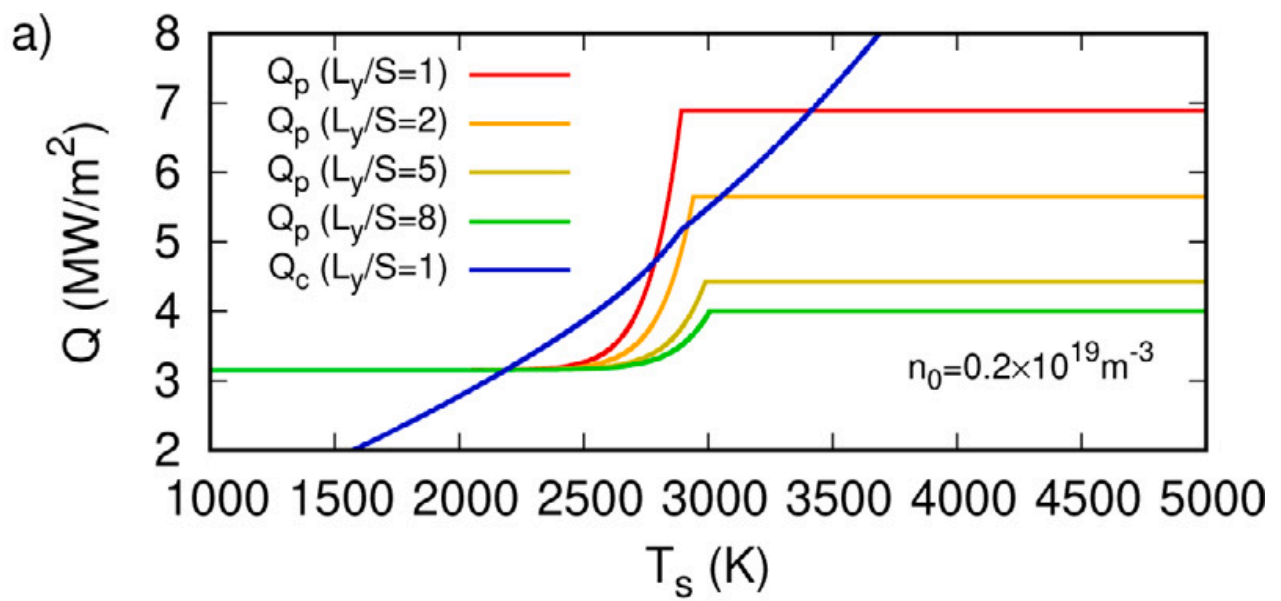
\includegraphics[width=0.7\linewidth]{material/Moritz_qTs.png}
    \caption[]{График зависимости плотности теплового потока на плитку от
    температуры поверхности плитки.~\cite{moritz2024simulated} Параметр $L_y/S$ --- отношение
площади пятна к площади всей поверхности плитки. $Q_p$ --- тепловой поток из
плазмы, $Q_c$ --- мощность теплоотвода, $n_0$ --- плотность плазмы}
	\label{pic::Moritz_qTs}
\end{figure}

\begin{figure}[H]
	\centering
	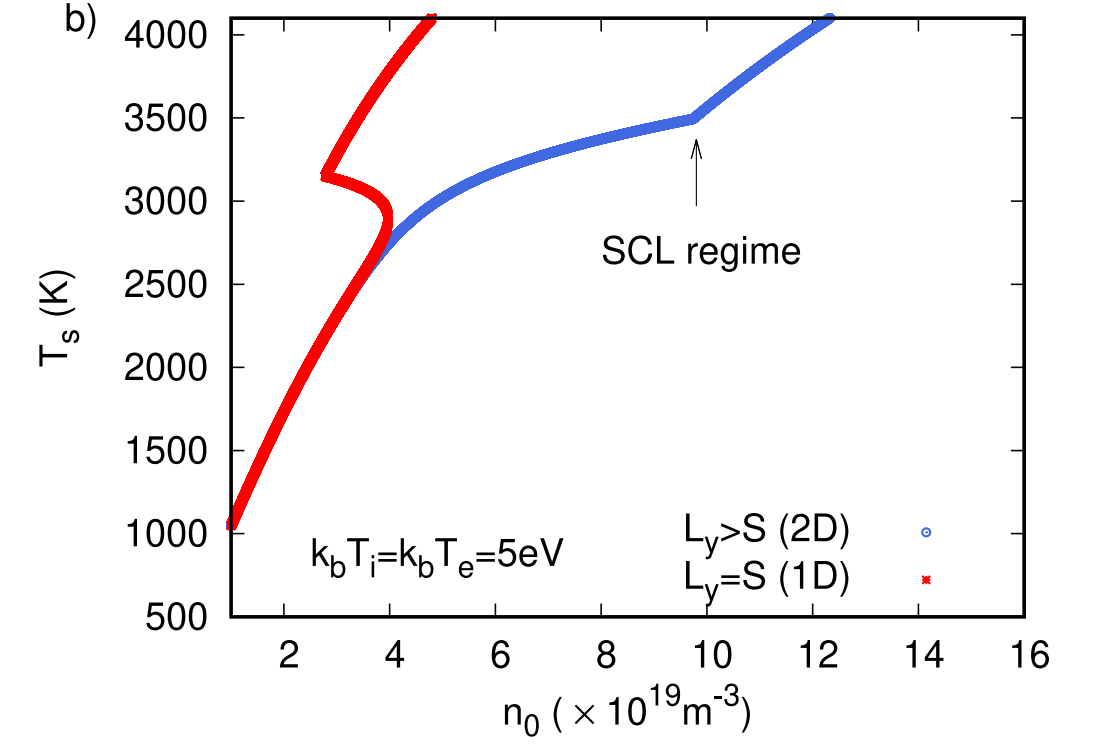
\includegraphics[width=0.7\linewidth]{material/Moritz_hysteresis.png}
    \caption[]{Пример кривой(красная кривая) гистерезиса зависимости
    стационарной температуры~\cite{moritz2024simulated}}
	\label{pic::Moritz_hysteresis}
\end{figure}

В результате PIC симуляций показано наличие осцилляций температуры поверхности
плитки и параметров систему ввиду инерции теплопроводности в материале. Так же 
показано существование ''запертых'' виртуальным катодом частиц.

Отметим\hl{допустимо ли множественное?}, что оценка~\eqref{eq::qClassicEstimate}
справедлива для локального термодинамического равновесия плазмы$\left(T_i =
T_e\right)$ и не учитывает наличия осцилляций электрического поля в дебаевском
слое, наблюдаемого в реальных экспериментах~\cite{kirk2006evolution}. Ввиду
нелинейного характера поведения дебаевского слоя, импеданс в среднем по периоду
осцилляций не равен нулю~\cite{myra2015radio}, что приводит к осцилляциям тока в
слое, и как следствие, тепловых потоков. В совокупности с наличием положительной
обратной связи в системе и инерцией теплопроводимости, это потенциально может
привести к значительному росту усреднённой по периоду осцилляций тепловой
нагрузки на стенку.
%

В современных работах изучено влияние множества факторов и составлены
соответствующие модели, учитывающие конечность
температуры ионов \cite{schwager1993effects}, ~\cite{ou2017heat}, отношения
температуры эмитированных электронов~\cite{sheehan2014effects}, наличие
фотоэлектронной эмиссии, отрицательных ионов~\cite{taccogna2014non}, различных
профилей распределения скоростей частиц~\cite{stangeby1984plasma},
пондеромоторных сил~\cite{takamura1998heat}, столкновительность
слоя~\cite{godyak2002smooth}\hl{и другие}.

Дебаевский слой является структурой с достаточно произвольной границей. Как
правило, принимается, что в данной точке поле равным нулю и справедлив критерий
Бома~\eqref{eq::Bohm_overview}.
\begin{equation}
    \upsilon_i^{se} \ge \sqrt{\cfrac{T_e + \gamma T_i}{m_e}}
    \label{eq::Bohm_overview}
\end{equation}

Однако предположение о равенстве поля на входе в слой является достаточно грубым
--- плазма начинает экранирует поле существующее в дебаевском слое на конечном
расстоянии. Так, в работе~\cite{godyak2002smooth} введено более общее
определение, основанное на данном замечании. В данной работе применяется
''классическое'' предположение о равенстве поля нулю на входе в слой.

Другая важная характеристика дебаевского слоя --- толщина, как правило
оценивается согласно классической формуле
Чайлда---Ленгмюра~\eqref{eq::Child_Langmuir_width}
\begin{equation}
    \lambda = \cfrac{1}{3\pi}\left(enV\right)^{-1/2}\left(\cfrac{2e}{m_e}\right)^{1/4}
    \label{eq::Child_Langmuir_width}
\end{equation}

Данная оценка так же сделана в достаточно грубых приближениях: в слое
отсутствуют электроны и начальная скорость ионов равна нулю. В
работе~\cite{chabert2014size} получена более точная оценка, учитывающая данные
факторы.\hl{графики}

Классический режим работы слоя известен давно и часто подразумевается при
использовании классических оценок теплового потока~\eqref{eq::qClassicEstimate}
и значения плавающего потенциала.~\hl{добавить работы}.

В работе~\cite{campanell2018alternative} рассматривается альтернативный
инвертированный режим работы слоя. В данной режиме слой монотонен, но
электростатический потенциал в дебаевском слое всюду больше потенциала плазмы.
Данный режим нестабилен относительно возмущений плотности, но имеет конечное
время релаксации к прежнему состоянию. В других работах автор
~\cite{campanell2016strongly},~\cite{campanell2020possible} отмечает, что
вообще говоря, режим объёмного экранирования зарядом не является устойчивым и
ввиду накопления ионов в промежутке между виртуальным катодом и поверхностью,
переходит в инвертированный режим. Данный режим обеспечивает \hl{''детачмент''}:
возле поверхности плитки образуется промежуточная область с холодной
плазмой.~\hl{подробнее о том зачем это}.

\pagebreak
